\section{Count-certificate construction and audit diagnostics}\label{app:audit}
Partition items into strata $h=1,\ldots,H$ before observing their audited
labels. Sample $n_h$ of the $M_h$ items without replacement. If $K_h$ is the
unknown number of incorrect predictions and $X_h$ the sampled error count,
then $X_h\sim\operatorname{Hypergeometric}(M_h,K_h,n_h)$. Assign nonnegative
error budgets $\delta_h$ with $\sum_h\delta_h\leq\delta$. Retain integers $K$
for which both $\Pr_K(X_h\leq x_h)\geq\delta_h/2$ and
$\Pr_K(X_h\geq x_h)\geq\delta_h/2$. Their extrema are $\ell_h,u_h$.
A census stratum has $\ell_h=u_h=x_h$; an unaudited stratum contributes no
count restriction.

Let $O$ be the audited items, $U_h$ the unaudited items in stratum $h$,
$c_j=(2q_j-1)w_j$, and $d_O=\sum_{j\in O}w_j(q_j-y_j)$. The smallest and
largest compatible errors are
\begin{align}
 L_A&=d_O+\sum_h\min_{\ell_h-x_h\leq m\leq u_h-x_h}
                 S_-(c_{U_h},m),\notag\\
 U_A&=d_O+\sum_h\max_{\ell_h-x_h\leq m\leq u_h-x_h}
                 S_+(c_{U_h},m).\label{eq:auditbounds}
\end{align}
The optimization is over integers. With signed weights, an extreme need not
occur at the largest admissible error count.

\begin{proof}[Proof of Proposition~\ref{prop:audit}]
Inverting each pair of hypergeometric tails excludes the true $K_h$ with
probability at most $\delta_h$. A union bound therefore includes all true
counts with probability at least $1-\delta$. On that event, the true errors in
$U_h$ number between $\ell_h-x_h$ and $u_h-x_h$. Sorting and choosing a count
in that range gives the extrema in equation~\eqref{eq:auditbounds}; the choices
are independent restrictions across strata and hence jointly attainable.
The true label vector lies in the same configuration set for every $w$, so the
coverage event applies simultaneously to all its linear contrasts.
\end{proof}
The labels and predictions are fixed under this design. Systematic or
correlated classifier mistakes do not invalidate coverage, which is over
repeated audit samples. The count region can be conservative, and sharp
projection of that region does not make its interval shortest. The guarantee
concerns one label vector; combining separate audits of several outcomes needs
an additional error allocation. Optional stopping, adaptive strata, and
imperfect audit labels require other procedures or assumptions.

\paragraph{Information lost by count projection.}
Let all $N$ predictions equal one, half the weights equal $1/N$ and half equal
$-1/N$. Suppose a fraction $p<1/2$ of labels in each half are wrong. The
true contrast is zero. If $n\to\infty$ but $n/N\to0$, an unstratified audit
consistently learns the overall error fraction. Yet unaudited errors can still
be placed almost entirely on either weight sign: the projected interval width
converges to $2p$. A direct estimate of the weighted audit residual instead
has standard error of order $n^{-1/2}$. Separating the two weight signs into
strata removes this particular information loss.

For a declared contrast, the stratified difference estimator uses
$z_j=w_j(y_j-q_j)$ directly:
\begin{equation}\label{eq:stratified}
 \widetilde\theta=\widehat\theta+
 \sum_h\frac{M_h}{n_h}\sum_{j\in O_h}z_j,\qquad
 \widehat V=\sum_h\frac{M_h^2(1-n_h/M_h)}{n_h}s_{z,h}^2.
\end{equation}
Under independent stratum draws, the estimate and variance estimator are
design unbiased when each noncensus stratum has at least two sampled items.
Normal intervals need a separate approximation. A conservative finite-sample
alternative applies Hoeffding's without-replacement inequality
\citep{hoeffding1963} to each bounded residual mean and sums the stratum
radii. More efficient weighted audit procedures exist
\citep{shekhar2023audits}.

\begin{figure}[htbp]
\centering
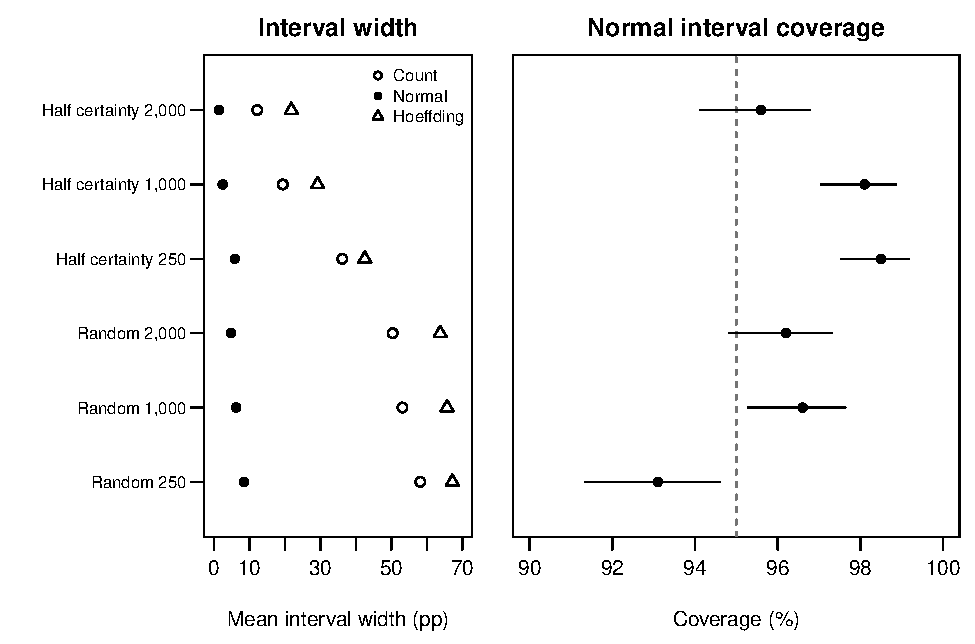
\includegraphics[width=\linewidth]{../figs/audit_comparison.pdf}
\caption{Width and coverage for the Facebook-pixel female share coefficient.
Rows compare audit budgets and designs in the fixed browsing frame. Left:
mean interval width in percentage points over 1,000 audits. Right: normal
interval coverage, with exact 95\% binomial Monte Carlo intervals and a dashed
95\% reference. Count and Hoeffding intervals covered in every simulated draw.
``Half certainty'' audits the largest absolute influences with half the budget.
Count intervals cover all contrasts of this outcome simultaneously; direct
intervals target this coefficient. The randomness is domain auditing; users
and predictions are fixed.}
\label{fig:audit}
\end{figure}

\begin{table}[htbp]
\centering\scriptsize
\caption{All audit designs and methods for the focal coefficient}
\label{tab:auditall}
\begin{tabular}{lrlrrrr}
\toprule
Design & Budget & Interval & Coverage (\%) & Width (pp; MCSE) & Correct sign (\%) & Wrong sign (\%) \\
\midrule
Random & 250 & Count projection & 100.0 & 58.2 (0.06) & 0.0 & 0.0 \\
Random & 250 & Direct normal & 93.1 & 8.4 (0.50) & 39.6 & 0.0 \\
Random & 250 & Direct Hoeffding & 100.0 & 67.2 (0.01) & 0.0 & 0.0 \\
Random & 1,000 & Count projection & 100.0 & 53.1 (0.05) & 0.0 & 0.0 \\
Random & 1,000 & Direct normal & 96.6 & 6.3 (0.19) & 32.9 & 0.0 \\
Random & 1,000 & Direct Hoeffding & 100.0 & 65.7 (0.02) & 0.0 & 0.0 \\
Random & 2,000 & Count projection & 100.0 & 50.4 (0.05) & 0.0 & 0.0 \\
Random & 2,000 & Direct normal & 96.2 & 4.8 (0.11) & 34.4 & 0.0 \\
Random & 2,000 & Direct Hoeffding & 100.0 & 63.8 (0.03) & 0.0 & 0.0 \\
Half certainty & 250 & Count projection & 100.0 & 36.2 (0.05) & 0.0 & 0.0 \\
Half certainty & 250 & Direct normal & 98.5 & 5.9 (0.29) & 40.6 & 0.0 \\
Half certainty & 250 & Direct Hoeffding & 100.0 & 42.5 (0.00) & 0.0 & 0.0 \\
Half certainty & 1,000 & Count projection & 100.0 & 19.4 (0.04) & 0.0 & 0.0 \\
Half certainty & 1,000 & Direct normal & 98.1 & 2.5 (0.04) & 41.9 & 0.0 \\
Half certainty & 1,000 & Direct Hoeffding & 100.0 & 29.2 (0.00) & 0.0 & 0.0 \\
Half certainty & 2,000 & Count projection & 100.0 & 12.2 (0.03) & 0.0 & 0.0 \\
Half certainty & 2,000 & Direct normal & 95.6 & 1.4 (0.01) & 65.0 & 0.0 \\
Half certainty & 2,000 & Direct Hoeffding & 100.0 & 21.8 (0.00) & 0.0 & 0.0 \\
\bottomrule
\end{tabular}

\par\smallskip
\begin{minipage}{\linewidth}\footnotesize
Each row summarizes 1,000 domain audits. Width is the mean in percentage
points, with its Monte Carlo standard error in parentheses. Sign columns
report exclusion of zero in the correct or wrong direction. All methods
within a design use the same draws. Exact binomial Monte Carlo intervals and
replicate results accompany the package.
\end{minipage}
\end{table}

The random and half-certainty designs were chosen for one coefficient. They do
not establish that this design is efficient for other contrasts. The count
certificate covered the target in every simulated draw but never excluded
zero. Direct normal intervals were much narrower, yet coverage in the smallest
random design fell below the nominal level. The finite-sample Hoeffding
baseline was wider than count projection. These comparisons do not identify a
finite-sample-valid, efficient direct interval for this design.

\begin{table}[htbp]
\centering\small
\caption{Refining validation strata for the focal coefficient}
\label{tab:refinement}
\begin{tabular}{rrrr}
\toprule
Strata & Exact-count width (pp) & Audit width (pp; MCSE) & Coverage (\%) \\
\midrule
2 & 49.7 & 53.2 (0.05) & 100.0 \\
10 & 34.7 & 47.1 (0.05) & 100.0 \\
50 & 21.8 & 48.2 (0.03) & 100.0 \\
\bottomrule
\end{tabular}

\par\smallskip
\begin{minipage}{\linewidth}\footnotesize
Rank bins of signed influence cross predicted labels. Exact-count width
conditions on the population count in every stratum; audit width averages
95\% count-projection intervals over 1,000 domain samples of size 1,000.
Width uncertainty is its Monte Carlo standard error. These partitions were
examined after the initial audit results. No design certified the sign.
\end{minipage}
\end{table}

The narrower exact-count range from finer strata need not translate into a
narrower audit interval: the fixed sample is divided among more strata and
the error budget is split across their discrete hypergeometric intervals.
The 10- versus 50-stratum mean-width difference should be read with the
reported Monte Carlo uncertainty, not as evidence of an optimal partition.
